\definecolor{zzttqq}{rgb}{0.6,0.2,0.}
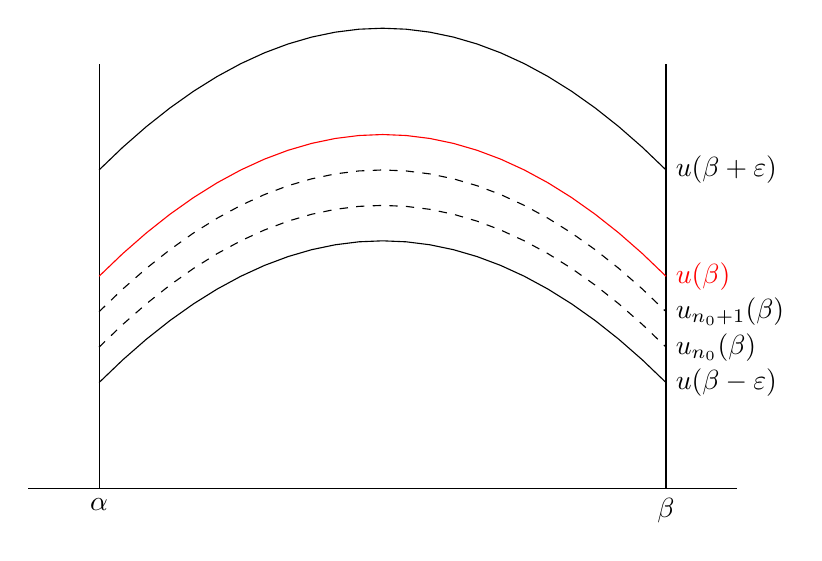
\begin{tikzpicture}[x=0.9cm,y=0.9cm]
\draw[color=black] (-1,0) -- (9,0);
\draw[color=black] (0,0) -- (0,6);
\draw[color=black] (8,0) -- (8,6);
\draw [domain=0:8, color=red] plot(\x,{-(1/8)*\x*\x+\x+3});
\draw [domain=0:8] plot(\x,{-(1/8)*\x*\x+\x+4.5});
\draw [domain=0:8] plot(\x,{-(1/8)*\x*\x+\x+1.5});
\draw [domain=0:8, dashed] plot(\x,{-(1/8)*\x*\x+\x+2.5});
\draw [domain=0:8, dashed] plot(\x,{-(1/8)*\x*\x+\x+2});
\draw[color=red] (8,3) node[anchor=west] {$u(\beta)$};
\draw (8,4.5) node[anchor=west] {$u(\beta+\varepsilon)$};
\draw (8,1.5) node[anchor=west] {$u(\beta-\varepsilon)$};
\draw (8,2) node[anchor=west] {$u_{n_0}(\beta)$};
\draw (8,2.5) node[anchor=west] {$u_{n_0+1}(\beta)$};
\draw (0,0) node[anchor=north] {$\alpha$};
\draw (8,0) node[anchor=north] {$\beta$};


\end{tikzpicture}